\input{./econtexRoot.texinput}
\documentclass[\econtexRoot/SequentialEGM]{subfiles}
\onlyinsubfile{\externaldocument{\econtexRoot/SequentialEGM}}
\usepackage{\econtexSetup,\econark,\econtexShortcuts}

\begin{document}

\hypertarget{higher-dimensions}{}
\par\section{The EGM$^n$ in Higher Dimensions}
\notinsubfile{\label{sec:higherdims}}

The problem in Section \ref{sec:method} demonstrates the simplicity of solving problems sequentially. However, as constructed, the problem has only one state variable and one post-decision state variable per stage. Can EGM$^n$ be used to solve higher dimensional problems? In short, yes, but it requires additional thought on interpolation.

\subsection{A more complex problem}

For a demonstration, we now turn to the problem of a worker saving up for retirement. This worker must consume, save, and deposit resources into a tax-advantaged account that can not be liquidated until retirement. In the recursive problem, the worker begins a new period with a liquid account of market resources $\mRat_{t}$ and an illiquid account of retirement savings $\nRat_{t}$. The worker maximizes their utility by choosing consumption $\cRat_{t}$ and pension deposit $\dRat_{t}$. The pension deposit is set aside on a retirement account that is exposed to a risky return, while their post-consumption liquid assets accrue risk-free interest every period. The worker additionally receives an income which faces a permanent ($\PGro_{t+1}$) and a transitory ($\tShkEmp_{t+1}$) shock every period. At the age of 65, the worker is retired and their assets are liquidated, at which point the state reduces to one liquid account of market resources. The worker's recursive problem is:

\begin{equation}
    \begin{split}
        \vFunc_{t}(\mRat_{t}, \nRat_{t}) & = \max_{\cRat_{t}, \dRat_{t}} \util(\cRat_{t}) + \DiscFac \Ex_{t} \left[ \PGro_{t+1}^{1-\CRRA} \vFunc_{t+1}(\mRat_{t+1}, \nRat_{t+1}) \right] \\
        & \text{s.t.} \quad \cRat_{t} \ge 0, \quad \dRat_{t} \ge 0 \\
        \aRat_{t} & = \mRat_{t} - \cRat_{t} - \dRat_{t} \\
        \bRat_{t} & = \nRat_{t} + \dRat_{t} + g(\dRat_{t}) \\
        \mRat_{t+1} & = \aRat_{t} \Rfree / \PGro_{t+1}  + \tShkEmp_{t+1} \\
        \nRat_{t+1} & = \bRat_{t} \Risky_{t+1} / / \PGro_{t+1}
    \end{split}
\end{equation}

where

\begin{equation}
    \gFunc(\dRat) = \xFer \log(1+\dRat).
\end{equation}

This problem can subsequently be broken down into 3 stages: a pension deposit stage, a consumption stage, and an income shock stage.

\subsection{Breaking down the problem}

In the deposit stage, the worker begins with market resources and a retirement savings account. The worker must maximize their value of liquid wealth $\lRat_{t}$ and retirement balance $\bRat_{t}$ by choosing a pension deposit $\dRat_{t}$, which must be positive. The retirement balance $\bRat$ is the cash-value of their retirement account plus their pension deposit and an additional amount $g(\dRat_{t})$ that provides an incentive to save for retirement. As we'll see, this additional term will allow us to use the endogenous grid method to solve this subproblem.

\begin{equation}
    \begin{split}
        \vFunc_{t}(\mRat_{t}, \nRat_{t}) & = \max_{\dRat_{t}} \vOpt_{t}(\lRat_{t}, \bRat_{t}) \\
        & \text{s.t.}  \quad \dRat_{t} \ge 0 \\
        \lRat_{t} & = \mRat_{t} - \dRat_{t} \\
        \bRat_{t} & = \nRat_{t} + \dRat_{t} + g(\dRat_{t})
    \end{split}
\end{equation}

After making their pension decision, the worker begins their consumption stage with liquid wealth $\lRat_{t}$ and retirement balance $\bRat_{t}$. From their liquid wealth, the worker must choose a level of consumption to maximize utility and continuation value $\wFunc_{t}$. After consumption, the worker is left with post-decision states that represent liquid assets $\aRat_{t}$ and retirement balance $\bRat_{t}$, which passes through this problem unaffected because it can't be liquidated until retirement.

\begin{equation}
    \begin{split}
        \vOpt_{t}(\lRat_{t}, \bRat_{t}) & = \max_{\cRat_{t}} \util(\cRat_{t}) + \DiscFac \wFunc_{t}(\aRat_{t}, \bRat_{t})  \\
        & \text{s.t.} \quad \cRat_{t} \ge 0 \\
        \aRat_{t} & = \lRat_{t} - \cRat_{t}
    \end{split}
\end{equation}

Finally, the post-decision value function $\wFunc_{t}$ represents the value of both liquid and illiquid account balances before the realization of uncertainty regarding the risky return and income shocks. Since we are dealing with a normalized problem, this stage handles the normalization of state variables and value functions into the next period.

\begin{equation}
    \begin{split}
        \wFunc_{t}(\aRat_{t}, \bRat_{t}) & = \Ex_{t} \left[ \PGro_{t+1}^{1-\CRRA} \vFunc_{t+1}(\mRat_{t+1}, \mRat_{t+1}) \right] \\
        & \text{s.t.} \quad \aRat_{t} \ge 0, \quad \bRat_{t} \ge 0 \\
        \mRat_{t+1} & = \aRat_{t} \Rfree / \PGro_{t+1}  + \tShkEmp_{t+1} \\
        \nRat_{t+1} & = \bRat_{t} \Risky_{t+1} /  \PGro_{t+1}
    \end{split}
\end{equation}

The advantage of conceptualizing this subproblem as a separate stage is that we can construct a function $\wFunc_{t}$ and use it in the prior optimization problems without having to worry about stochastic optimization and taking expecations repeatedly.

\subsection{The consumption-saving problem}

As seen in the consumption stage above, the retirement balance $\bRat_{t}$ passes through the problem unaffected because it can't be liquidated until retirement. In this sense, it is already a post-decision state variable. To solve this problem, we can use a fixed grid of $\bRat_{t}$ and for each obtain endogenous consumption and ex-ante market resources using the simple endogenous grid method for the consumption problem.

\subsection{The pension deposit problem}

In the deposit stage, both the state variables and post-decision variables are different since both are affected by the pension deposit decision.

First, we can rewrite the pension deposit problem more compactly as:

\begin{equation}
    \vFunc_{t}(\mRat_{t}, \nRat_{t}) = \max_{\dRat_{t}}
    \vOpt_{t}(\mRat_{t}
    - \dRat_{t}, \nRat_{t} + \dRat_{t} + \gFunc(\dRat_{t}))
\end{equation}

The first order condition is

\begin{equation}
    \vOpt_{t}^{\lRat}(\lRat_{t}, \bRat_{t})(-1) +
    \vOpt_{t}^{\bRat}(\lRat_{t}, \bRat_{t})(1+\gFunc'(\dRat_{t})) = 0.
\end{equation}

Rearranging this equation gives

\begin{equation}
    \gFunc'(\dRat_{t}) = \frac{\vOpt_{t}^{\lRat}(\lRat_{t},
        \bRat_{t})}{\vOpt_{t}^{\bRat}(\lRat_{t}, \bRat_{t})} - 1
\end{equation}

where

\begin{equation}
    \gFunc'(\dRat) =
    \frac{\xFer}{1+\dRat} \qquad \gFunc'^{-1}(y) = \xFer/y - 1
\end{equation}

Given that $\gFunc'(\dRat)$ exists and is invertible, we can find

\begin{equation}
    \dEndFunc_{t}(\lRat_{t}, \bRat_{t}) = \gFunc'^{-1}\left(
    \frac{\vOpt_{t}^{\lRat}(\lRat_{t},
        \bRat_{t})}{\vOpt_{t}^{\bRat}(\lRat_{t},
        \bRat_{t})} - 1 \right)
\end{equation}

Using this, we can back out $\nRat_{t}$ as

\begin{equation}
    \nEndFunc_{t}(\lRat_{t}, \bRat_{t}) = \bRat_{t} -
    \dEndFunc_{t}(\lRat_{t}, \bRat_{t}) - \gFunc(\dEndFunc_{t}(\lRat_{t},
        \bRat_{t}))
\end{equation}

and $\mRat_{t}$ as

\begin{equation}
    \mEndFunc_{t}(\lRat_{t}, \bRat_{t}) = \lRat_{t} +
    \dEndFunc_{t}(\lRat_{t}, \bRat_{t})
\end{equation}

In sum, given an exogenous grid $(\lRat_{t}, \bRat_{t})$ we obtain the triple
$\left(\mEndFunc_{t}(\lRat_{t}, \bRat_{t}), \nEndFunc_{t}(\lRat_{t},
        \bRat_{t}), \dEndFunc_{t}(\lRat_{t}, \bRat_{t})\right)$, which
we can use to
create an interpolator for the decision rule $\dRat_{t}$.

To close the solution method, the envelope conditions are

\begin{equation}
    \begin{split}
        \vFunc_{t}^{\mRat}(\mRat_{t}, \nRat_{t}) & =
        \vOpt_{t}^{\lRat}(\lRat_{t}, \bRat_{t}) \\
        \vFunc_{t}^{\nRat}(\mRat_{t}, \nRat_{t}) & =
        \vOpt_{t}^{\bRat}(\lRat_{t}, \bRat_{t})
    \end{split}
\end{equation}

\subsection{Unstructured Grid Interpolation}

As in Section \ref{sec:method}, the resulting endogenous grid is not rectilinear, and in this more complex problem it is not even a regular grid. We can see in Figure \ref{fig:exog} that starting from a regular and rectilinear exogenous grid of liquid assets post-consumption $\lRat_{t}$ and pension balances post-deposit $\bRat_{t}$, we obtain Figure \ref{fig:endog} which shows an irregular and unstructured endogenous grid of market resources $\mRat_{t}$ and pension balances pre-deposit $\nRat_{t}$.

\begin{figure}
    \centering
    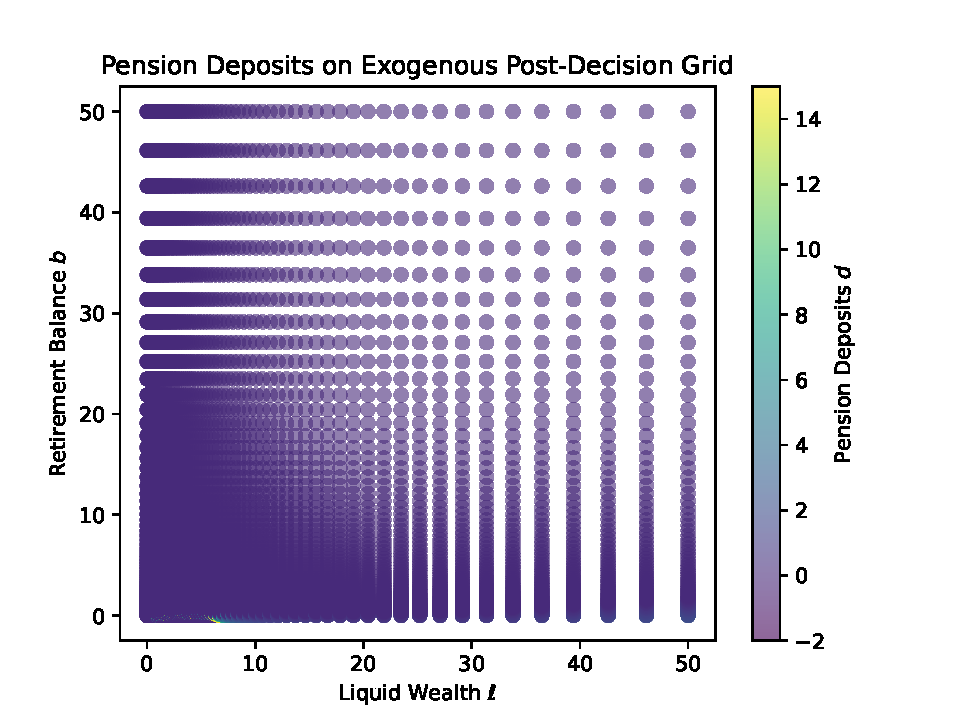
\includegraphics[width=0.8\linewidth]{Figures/ExogenousGrid.pdf}
    \caption{A regular, rectilinear exogenous grid of pension balances after deposit $\bRat_{t}$ and liquid assets after consumption $\lRat_{t}$.}
    \notinsubfile{\label{fig:exog}}
\end{figure}

\begin{figure}
    \centering
    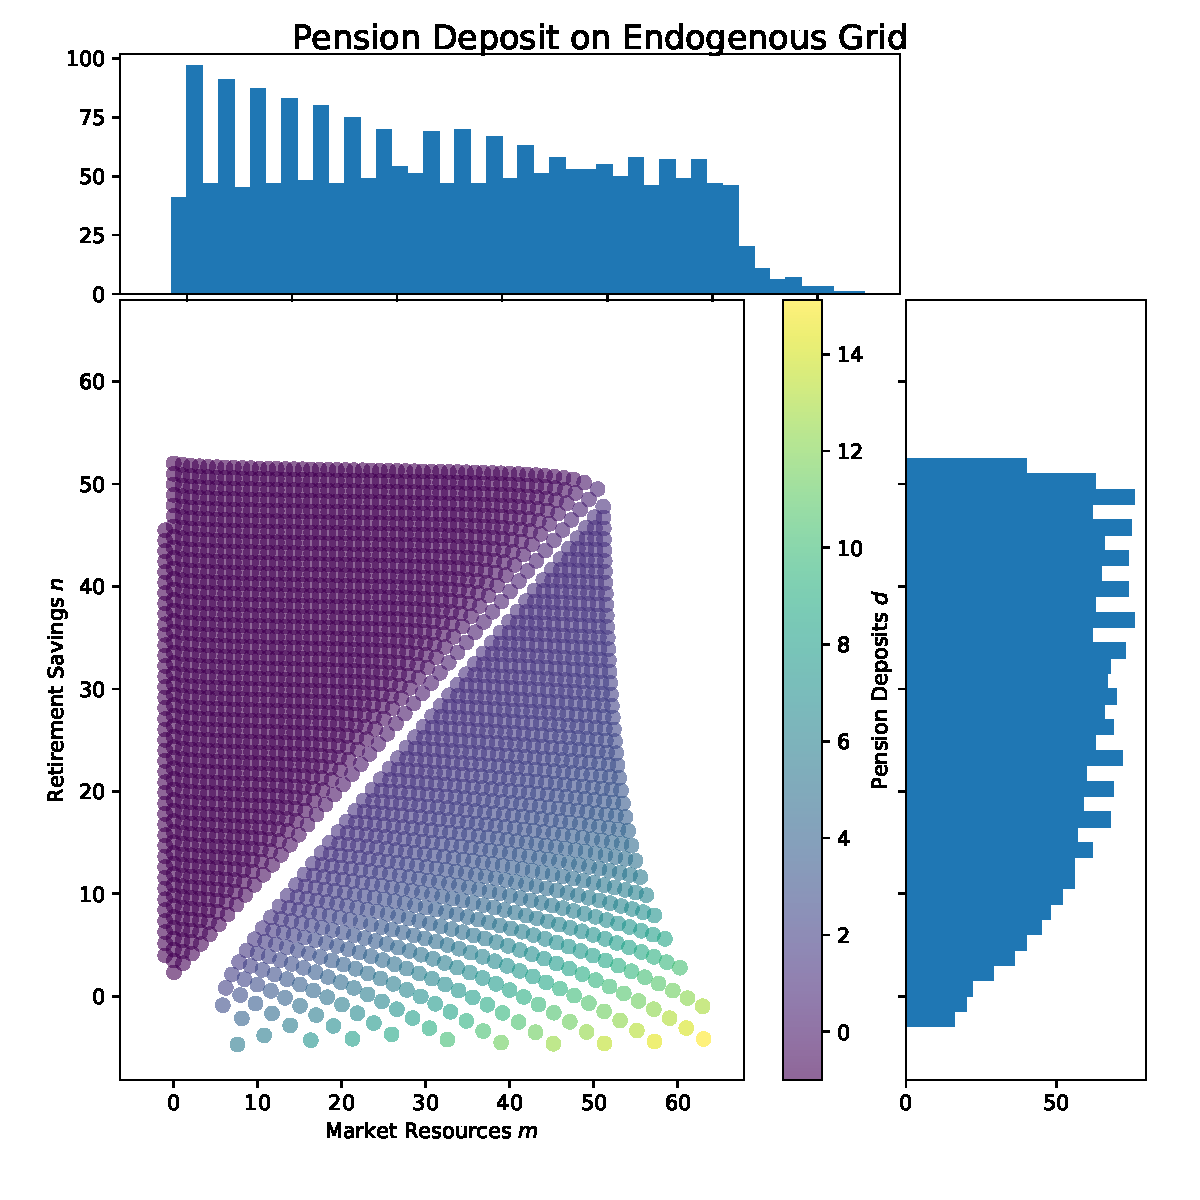
\includegraphics[width=0.8\linewidth]{Figures/EndogenousGrid.pdf}
    \caption{An irregular, unstructured endogenous grid of market resources $\mRat_{t}$ and pension balances before deposit $\nRat_{t}$.}
    \notinsubfile{\label{fig:endog}}
\end{figure}

To interpolate a function defined on an unstructured grid, we use Gaussian Process Regression as in \cite{Scheidegger2019-xf}.

\ifthenelse{\boolean{Web}}{}{
\end{document} \endinput
}
